%\documentclass[12pt]{article}
%\usepackage[margin=1 in, head=0.9 in]{geometry}
%\usepackage{fancyhdr}
%\usepackage{listings}
%\usepackage{caption}
%\usepackage{color}
%\usepackage{xcolor}
%\usepackage{caption, apacite}
%\DeclareCaptionFont{white}{\color{white}}
%\DeclareCaptionFormat{listing}{\colorbox{gray}{\parbox{\textwidth}{#1#2#3}}}
%\captionsetup[lstlisting]{format=listing,labelfont=white,textfont=white}
%\usepackage{graphicx}
%\usepackage{amsmath, amssymb, amsthm}
%\usepackage[all,cmtip]{xy}
%\pagestyle{fancy}
\input{/home/dmitry/Work/Research/thesis/FINALE/settings.tex}

\begin{document}

\title{Scattering of tsunami waves by Koko Guoyt}
\maketitle

\section*{Abstract}
Tsunami waves as shallow gravity waves feel the bottom such that the incident energy can be scattered. Example of such interaction is Koko Guoyt scattering of tsunami waves originating at Japan-Kuril trench. As the waves encounter elliptic guoyt, the wave energy organizes into tight beams with strong directional and temporal characteristic. This is shown by investigation of energetics in two recent tsunami events, Kuril 2006 and Tohoku 2011. These events have shown distinctive signature in Crescent City by strong secondary waves lagging after the first wave. The analytic solution developed proves that the secondary waves are a result of scattering by Koko Guyot. This mechanism has selective property that depends on incidence of the initial tsunami wave packet. For tsunami waves originating at Kuril trench scattering amplifies higher frequencies while for more direct incidence from Japan trench - longer frequencies are preferred.

\section{Introduction}
Tsunami wave as being extreme example of shallow gravity waves transverse the ocean basins in a number of hours. Since the ocean basins are usually consist of inhomogeneities associated with submarine topographic features, the tsunami energy becomes dispersed and scattered (\cite{mofjeld2001tsunami}). In the opposite cases diffraction over shallow seamounts creates focused ``energy rays" (\cite{tang2012direct}, \cite{dushaw2015empirical}.\\
Interaction of tsunami waves with underlying bathymetry creates spatial and temporal differences. This was observed for recent tsunami events, Kuril tsunami of November 2006 (\cite{kowalik2008kuril}) and Tohoku event (\cite{allan2012march}). In both cases, tsunami arrival to the West coast was enhanced in the Northern California. Additionally, the maximum amplitude was observed after the first waves. Such characteristics of tsunami is attributed to scattering of tsunami by Emperor seamountains and Hess Rise and consequent energy trapping by Mendocino Escarpment (\cite{kowalik2008kuril}, \cite{rasmussen2015source}). Here it will be addressed how the largest seamountain, Koko Guoyt, in the chain affects tsunami. oko guyot (Figure 1) is a seamount in Emperor seamountain chain. It emerges from the surrounding abyssal plane of 5500 meters to 300 meters over distance in 20-30 km. The upper part has a distinct plateau with mean depth 800 m and elliptical shape with semimajor axis of 65 km and semiminor - 25 km.\\
Since tsunami waves comprise large number of different frequencies it is hypothesized that the response of Koko guoyt is frequency dependent. As well, it is notable that due to shape of the seamountain response will also depend on incident angle of the waves. This is a similar to resonance of Hawaii islands (\cite{munger2008resonance}) or shelf (\cite{yamazaki2011shelf}).\\
We start by comparison of two numerically simulated events where the differences of tsunami wave are characterized (Section 2). Than by carrying out frequency analysis and developing patterns for energy transports around Koko Guoyt we develop physical insights into the problem These are further supported by a simple analytical model of harmonic wave interaction with an elliptic seamount. And further we conclude our work.

\begin{figure}[h]
\centering
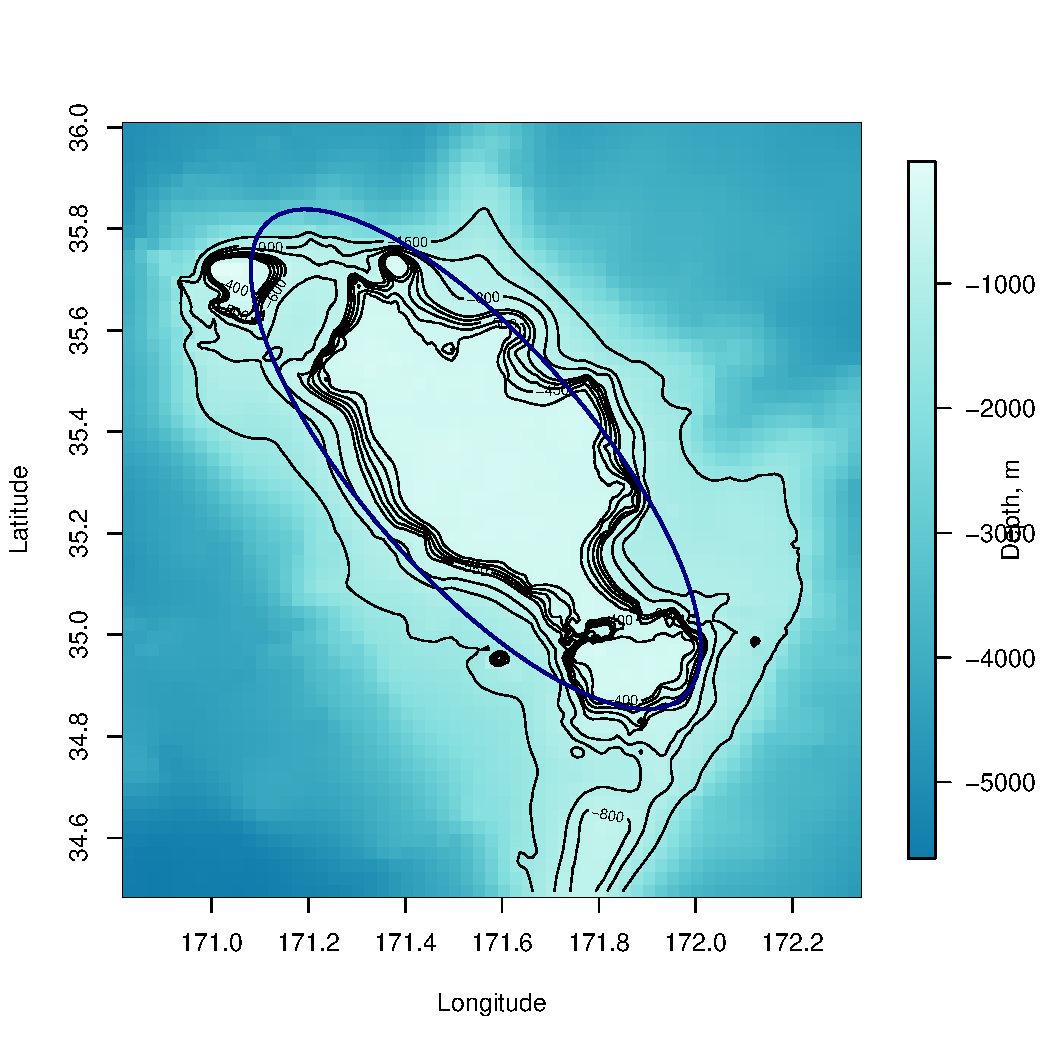
\includegraphics[scale=0.5]{../figures/koko_ell.pdf}
\end{figure}

\section{Numerical simulations and characteristics of Kuril November event, 2006 and Tohoku tsunami event, 2011}
\subsection{Numerical simulation}
Tsunami wave packet consists of many frequencies (fig. 2). Notable that most of the energy is associated with waves in range of minutes to one hour.
\begin{figure}
\mfig[0.5]{tsunami_spectra.pdf}
\mfig[0.5]{spectra_tsunami_21414.pdf}
\caption{a) FFT of tsunami wave observed at DART station 21418 close to Japan after Tohoku event in 2011. b) Same for station 21414 after Kuril tsunami in November 2006.}
\end{figure}
In this investigation as well two tsunami events are kept in mind. The first tsunami was triggered by prominent earthquake in Japan, in March 2011. The second event happened due to Kuril earthquake in Novermber 2006. To investigate differences in wave-bathymetry interaction using ray tracing are found difference in wave incidence (Figure 2). It is clear the waves from the first event had more East-West direction while for Kuril event the waves approached Koko Guyot from Northwest.
\begin{figure}
\mfig[0.5]{koko_rays.pdf}
\caption{Comparison of wavelength and seamountain sizes following dispersion relation for the surface waves (all done on fingers, so REDO picture)}
\end{figure}
Secondary waves...
\subsection{Frequency analysis}
We apply tf-method to understand what the changes were occurring in tsunami waves over time.

\subsection{Energetics}
We calculate energy fluxes
\begin{figure}
\mfig[0.5]{fluxes_exps_total.png}
\end{figure}
effect on CC looks like this,
\begin{figure}
\mfig[0.5]{cc_inc_flux.png}
\end{figure}

\section{Scattering by Koko Guoyt}
\subsection{Numerical results}
\begin{figure}
\mfig[0.5]{fluxes_exps_examp.png}
\end{figure}

\subsection{Analytical model}

\section{Discussion and Conclusions}

\newpage


\bibliographystyle{apacite}
\bibliography{/home/dmitry/Bibtex_lib/my_first_lib}

\end{document}